\documentclass[12pt,a4paper]{article}

% Language and encoding
\usepackage[french]{babel}
\usepackage[utf8]{inputenc}
\usepackage[T1]{fontenc}

% Page size and margins
\usepackage[a4paper,top=2cm,bottom=2cm,left=3cm,right=3cm]{geometry}

% Packages for titlepage, toc, graphics, tables, math, hyperlinks
\usepackage{titling}
\usepackage{graphicx}
\usepackage{amsmath,amsfonts,amssymb}
\usepackage{booktabs}
\usepackage[colorlinks=true, allcolors=blue]{hyperref}
\usepackage{float}

% Bibliography
\usepackage{biblatex}
\addbibresource{references.bib}

% Header/Footer
\usepackage{fancyhdr}
\pagestyle{fancy}
\fancyhf{}
\rhead{\leftmark}
\lhead{Projet SDD}
\rfoot{\thepage}

% Title page data
\title{Analyse de la dépense calorique en séance de sport}
\author{
  Rémi MALAPERT \\
  Othmane NAMMOUS \\
  Tharushan UTHAYAKUMAR
}
\date{20 mai 2025}

\begin{document}

%====================
% Page de garde
%====================
\begin{titlepage}
\centering
\vspace*{2cm}
{\LARGE\bfseries Analyse de la dépense calorique
en séance de sport\par}
\vspace{1.5cm}
{\large Projet de Sciences des Données\\
Encadré par Monsieur \href{https://antonio-ocello.github.io/}{Antonio Ocello}, post-doctorant au \href{https://cmap.ip-paris.fr/}{CMAP}, École Polytechnique\par}
\vspace{2.5cm}
{\large
Rémi Malapert \
Othmane Nammous \
Tharushan Uthayakumar\par}
\vfill
{\large \today\par}
\end{titlepage}

%====================
% Résumé (Abstract)
%====================
\begin{abstract}
Ce rapport détaille l’analyse statistique et la modélisation de la dépense calorique
lors de séances de sport à partir du \href{https://www.kaggle.com/datasets/valakhorasani/gym-members-exercise-dataset}{Gym Members Exercise Dataset} (973 observations).
Après nettoyage et standardisation des variables continues (âge, poids, IMC, fréquence cardiaque, etc.),
plusieurs modèles de régression linéaire multiple ont été ajustés, diagnostiqués et comparés
via AIC, BIC et validation croisée. Les résultats soulignent les variables les plus influentes
et aboutissent à un modèle parcimonieux expliquant plus de 50\% de la variance de la dépense
calorique. Les diagnostics (résidus, leverage, distance de Cook, VIF) confirment la validité
des hypothèses de régression, et la conclusion propose des recommandations pour un entraînement
personnalisé.
\end{abstract}

\newpage

%====================
% Table des matières
%====================
\tableofcontents
\newpage

%====================
% 1. Introduction
%====================
\section{Introduction}
Le choix du \emph{Gym Members Exercise Dataset} se fonde sur son jeu de 973 sessions riche et homogène, et sur son taux d’usability élevé, qui facilite l’importation et l’analyse des données. Le sport constitue un sujet d’intérêt pour le groupe, et, alors que deux d’entre nous suivent la spécialité « santé », nous souhaitons quantifier l’influence des paramètres continus (âge, poids, IMC, fréquence cardiaque moyenne, pourcentage de masse grasse) sur le nombre de calories brûlées pendant une séance.

Cette étude s’organise en trois volets : (1) un prétraitement des données pour ne conserver que les variables continues pertinentes et assurer leur comparabilité, (2) une modélisation par régression linéaire multiple avec sélection de variables selon leur significativité et les critères d’information (AIC, BIC), (3) des diagnostics détaillés (résidus, leverage, distance de Cook, VIF) et une validation croisée k–fold pour évaluer la robustesse prédictive du modèle. Nous terminons par une discussion des résultats et des recommandations pour adapter les entraînements en fonction des profils physiologiques identifiés.


\section{Contexte et objectifs}

\subsection{Problématique}
Comment quantifier et prévoir la dépense calorique pendant une séance de sport, en s’appuyant exclusivement sur les variables quantitatives (âge, poids, IMC, mesures cardiaques, pourcentage de masse grasse, etc.) ?

\subsection{Contraintes}
\begin{itemize}
    \item Exclusion des variables catégorielles (genre, type d’entraînement, fréquence hebdomadaire, durée des sessions, expérience).
    \item Préservation de l’interprétation de la variable cible (calories en kcal).
    \item Priorité à la parcimonie (modèles courts faciles à expliquer).
\end{itemize}


\section{Description et préparation des données}

\subsection{Sélection et nettoyage}
\textbf{Variables retenues (973 observations)}:
\begin{itemize}
    \item \texttt{Age, Weight (kg), Height (m), Max\_BPM, Avg\_BPM, Resting\_BPM,\\ Fat\_Percentage, Water\_Intake, BMI, Calories\_Burned}
\end{itemize}

\textbf{Imputation}:
Le jeu de données ne contenait aucune valeur manquante.

\textbf{Détection des outliers}:
Application conjointe de la méthode IQR (points hors des bornes [Q1 – 1.5×IQR, Q3 + 1.5×IQR]) et du Z-score (|Z| > 3) pour repérer et documenter les observations extrêmes avant toute modélisation.

\begin{figure}[H]
  \centering
  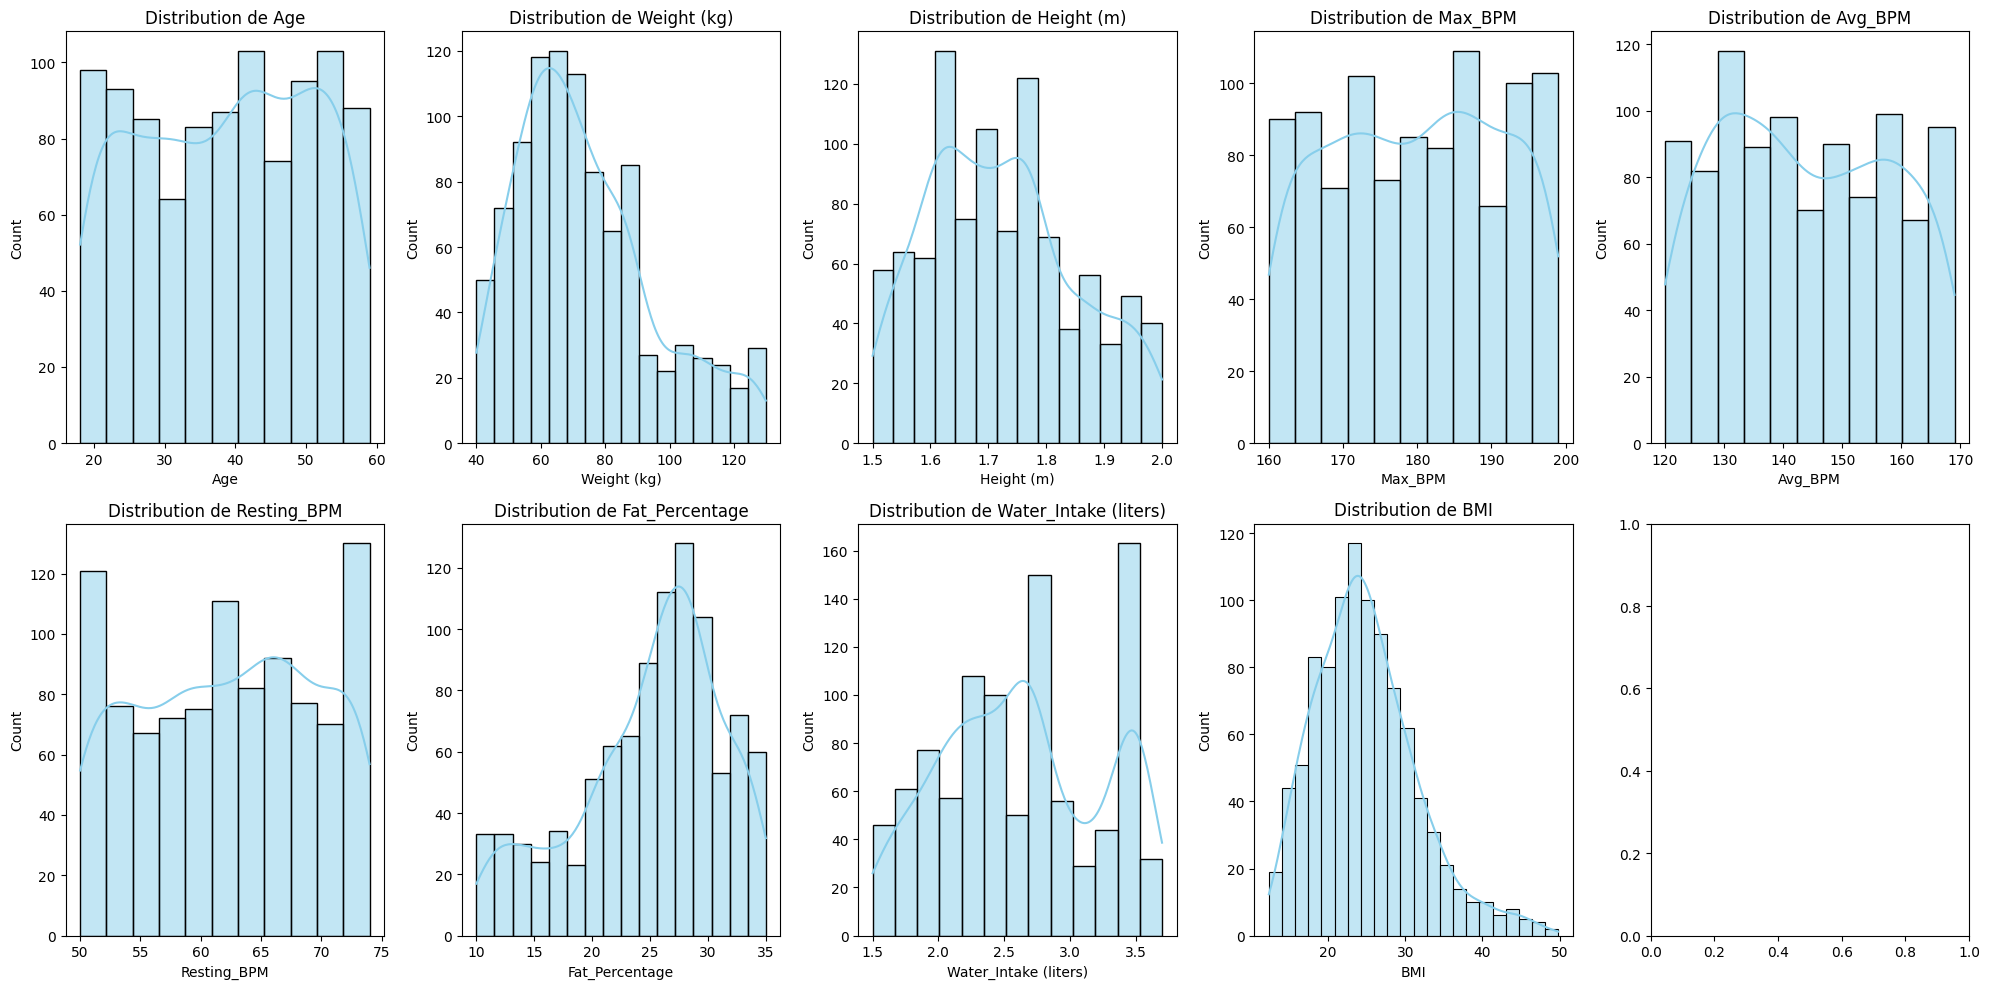
\includegraphics[width=0.7\linewidth]{distribution.png}
  \caption{Distribution des variables continues}
\end{figure}

\begin{figure}[H]
  \centering
  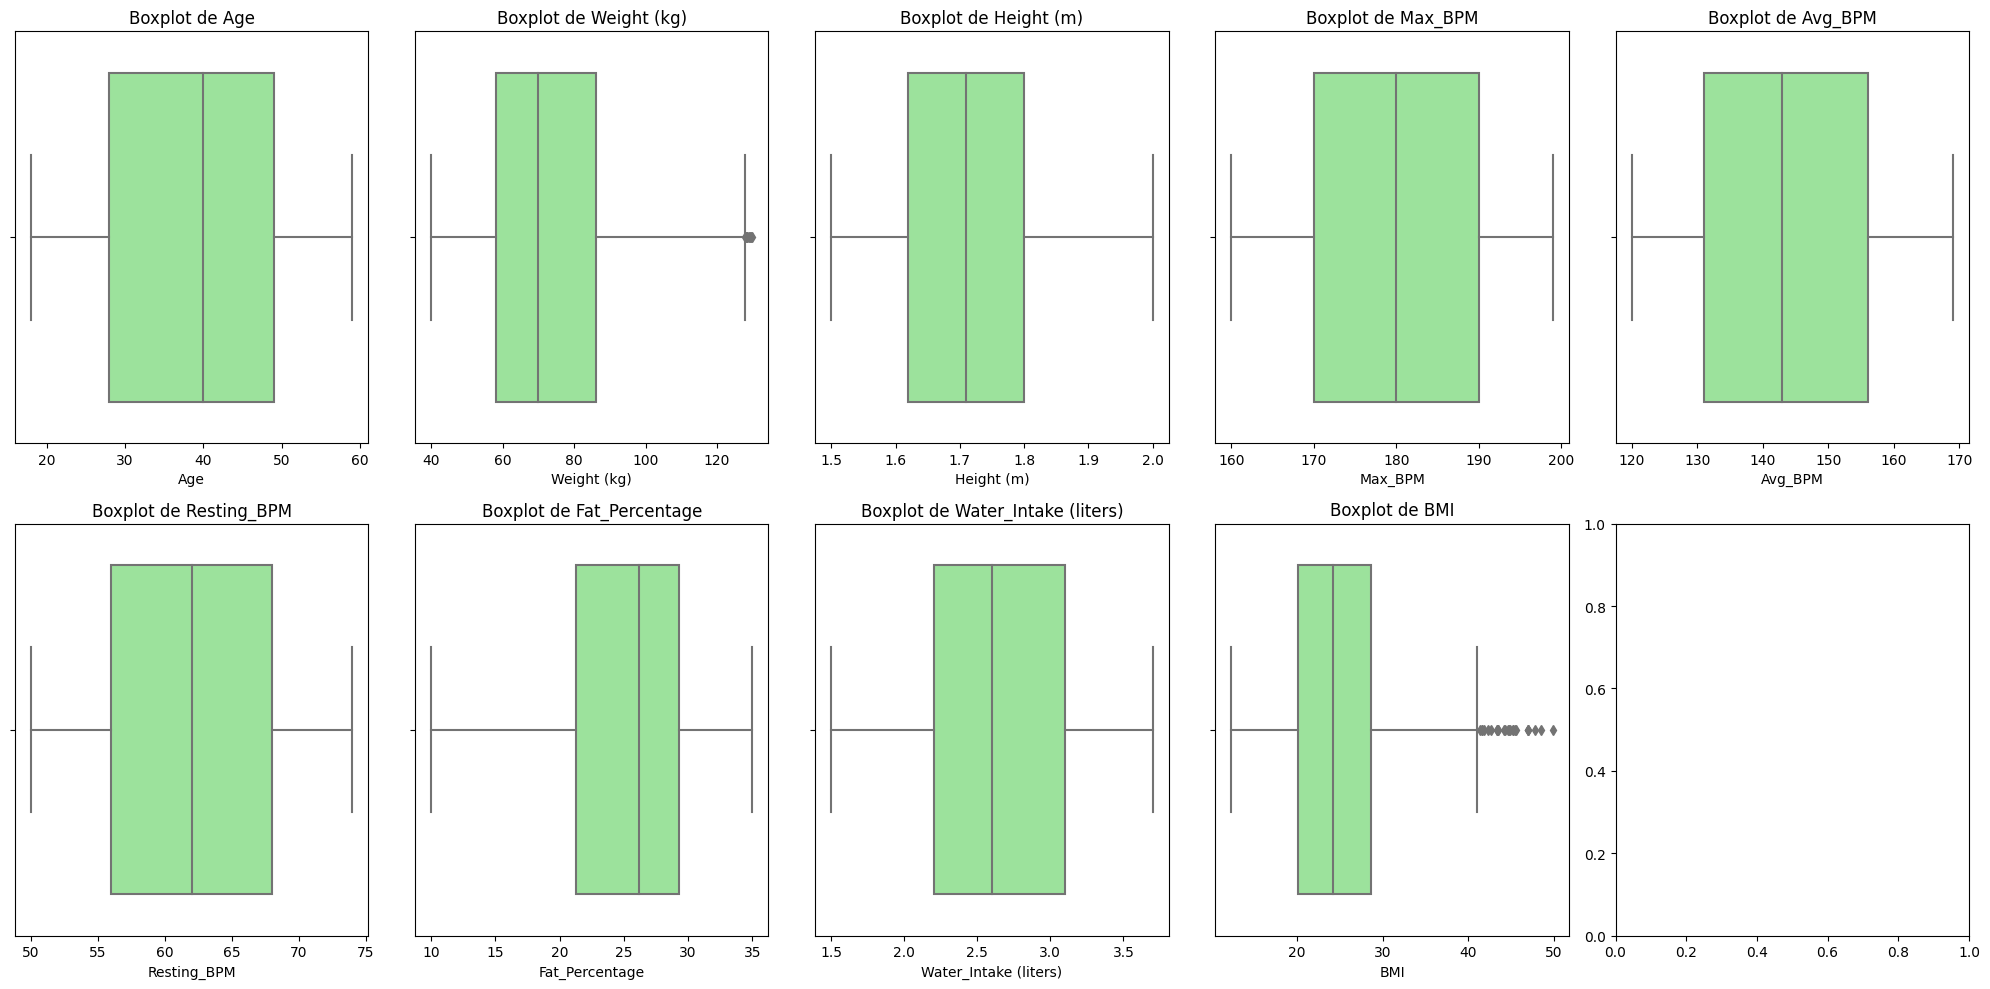
\includegraphics[width=0.7\linewidth]{boxplot.png}
  \caption{Boxplot des variables continues}
\end{figure}

\subsection{Standardisation}
\textbf{But}:
Mettre les prédicteurs sur une même échelle (moyenne = 0, écart-type = 1) afin que les coefficients soient directement comparables en termes d’impact relatif.

\textbf{Exception}:
La variable cible, \texttt{Calories\_Burned}, reste en unité absolue pour que les métriques d’erreur (RMSE, MAE) gardent leur sens opérationnel (kcal).


\section{Exploration initiale}

\subsection{Distributions univariées}
Historiques et boxplots montrent que la plupart des variables (poids, IMC, calories) sont légèrement asymétriques, ce qui justifie la vigilance quant aux outliers.

\subsection{Corrélations}
La matrice de corrélation met en évidence :
\begin{itemize}
    \item Corrélation forte entre \texttt{Fat\_Percentage} et \texttt{BMI} ($r = 0{,}75$).
    \item Corrélation modérée entre \texttt{Avg\_BPM} et \texttt{Calories\_Burned} ($r = 0{,}45$).
    \item Faible corrélation entre \texttt{Weight} et \texttt{Calories\_Burned}, ainsi qu’entre \texttt{Height} et \texttt{Calories\_Burned}, une fois les autres variables contrôlées.
\end{itemize}


\begin{figure}[H]
  \centering
  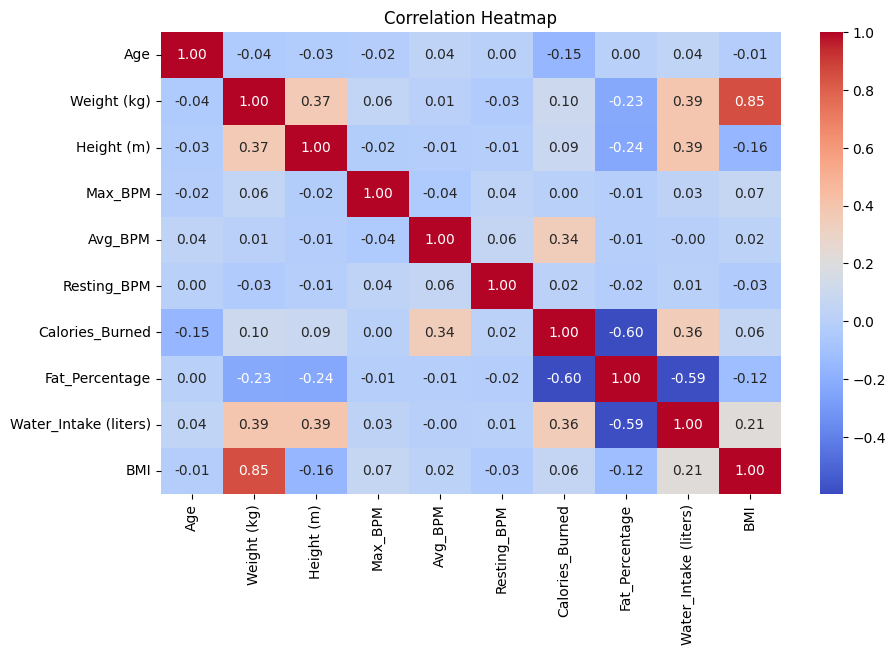
\includegraphics[width=0.7\linewidth]{correlation.png}
  \caption{Matrice de corrélation}
\end{figure}

\section{Modélisation initiale et diagnostic}

\subsection{Principe de la régression linéaire multiple}

On dispose d’un jeu de données de \(n\) observations \(\{(x_{i1}, x_{i2}, \dots, x_{ip}, y_i)\}_{i=1}^n\), où \(y\) est la variable à expliquer et \(\{x_j\}_{j=1}^p\) sont les \(p\) variables explicatives continues. On cherche à ajuster le modèle linéaire suivant :
\[
y_i \;=\;\beta_0 + \beta_1\,x_{i1} + \beta_2\,x_{i2} + \cdots + \beta_p\,x_{ip} + \varepsilon_i,
\]
avec \(\varepsilon_i\) un terme d’erreur supposé centré (\(\mathbb{E}[\varepsilon_i]=0\)) et de variance constante (\(\mathrm{Var}(\varepsilon_i)=\sigma^2\)), indépendant et identiquement distribué.

En notation matricielle :
\[
\mathbf{y} = X\,\boldsymbol{\beta} + \boldsymbol{\varepsilon},
\]
où
\[
\mathbf{y} = 
\begin{pmatrix}
y_1 \\ y_2 \\ \vdots \\ y_n
\end{pmatrix},\quad
X = 
\begin{pmatrix}
1 & x_{11} & x_{12} & \cdots & x_{1p} \\
1 & x_{21} & x_{22} & \cdots & x_{2p} \\
\vdots & \vdots & \vdots & \ddots & \vdots \\
1 & x_{n1} & x_{n2} & \cdots & x_{np}
\end{pmatrix},\quad
\boldsymbol{\beta} = 
\begin{pmatrix}
\beta_0 \\ \beta_1 \\ \vdots \\ \beta_p
\end{pmatrix}.
\]

Les coefficients \(\boldsymbol{\beta}\) sont estimés par la méthode des moindres carrés ordinaires (OLS), minimisant la somme des carrés des résidus :
\[
\hat{\boldsymbol{\beta}}
= \arg\min_{\boldsymbol{\beta}}
(\mathbf{y} - X\boldsymbol{\beta})^\top(\mathbf{y} - X\boldsymbol{\beta})
\;\;\implies\;\;
\hat{\boldsymbol{\beta}} = (X^\top X)^{-1} X^\top \mathbf{y}.
\]

L’ajustement du modèle est ensuite évalué à l’aide de plusieurs indicateurs :
\begin{itemize}
  \item Le coefficient de détermination \(R^2 = 1 - \tfrac{\mathrm{SS}_{\mathrm{rés}}}{\mathrm{SS}_{\mathrm{tot}}}\), qui mesure la proportion de la variance expliquée.
  \item Le \(R^2\) ajusté, qui pénalise l’ajout de variables non informatives :
    \[
      R^2_{\mathrm{ajusté}} = 1 - (1-R^2)\,\frac{n-1}{n-p-1}.
    \]
  \item Les tests de significativité (statistiques \(t\) pour chaque \(\beta_j\), test global \(F\)).
  \item Les diagnostics de résidus et d’influence (qui vérifient l’homoscédasticité, la normalité des \(\varepsilon_i\), la présence de points influents, etc.).
\end{itemize}

\subsection{Régression linéaire multiple complète}
\textbf{Résultats clés}:
\begin{itemize}
    \item R² = 0,50 (50\% de la variance expliquée).
    \item AIC/BIC élevés, F-statistic \begin{math}p < {10}^{-10}.\end{math}
    \item Variables significatives (\(p < 0,05\)) : \texttt{Age}, \texttt{Avg\_BPM}, \texttt{Fat\_Percentage}, \texttt{Water\_Intake}.
\end{itemize}

\subsection{Multicolinéarité}
\textbf{VIF}:
\begin{itemize}
    \item \texttt{Weight} : VIF = 70 ; \texttt{Height} : VIF = 20 ; \texttt{BMI} : VIF = 64 → colinéarité extrême.
\end{itemize}

\textbf{Décision}:
Exclusion de \texttt{Weight} et \texttt{BMI}, puis réévaluation.

\subsection{Modèle sans variables colinéaires}
Ajout des prédicteurs \{\texttt{Age}, \texttt{Avg\_BPM}, \texttt{Resting\_BPM}, \texttt{Fat\_Percentage}, \texttt{Water\_Intake}, \texttt{BMI}\}

\textbf{Résultats}:
\begin{itemize}
    \item VIF retombent tous < 2
    \item R² = 0,50, adj-R² = 0,49 → quasi-identique au modèle complet, diagnostic sensiblement plus stable.
\end{itemize}

\section{Diagnostics approfondis}

\begin{table}[H]
  \centering
  \caption{Résultats des tests de diagnostic}
  \begin{tabular}{ll}
  \toprule
  \textbf{Test / Graphique} & \textbf{Valeur / Observation} \\
  \midrule
  QQ-plot              & Alignement satisfaisant sur la diagonale (normalité quasi-respectée) \\
  Leverage (\(h_i\))   & Aucun point au-dessus de \(\tfrac{3(p+1)}{n}\) (p = 3) \\
  Cook’s D             & Toutes les distances < 0,5 → pas de points influents majeurs \\
  \bottomrule
  \end{tabular}
\end{table}

\begin{figure}[H]
  \centering
  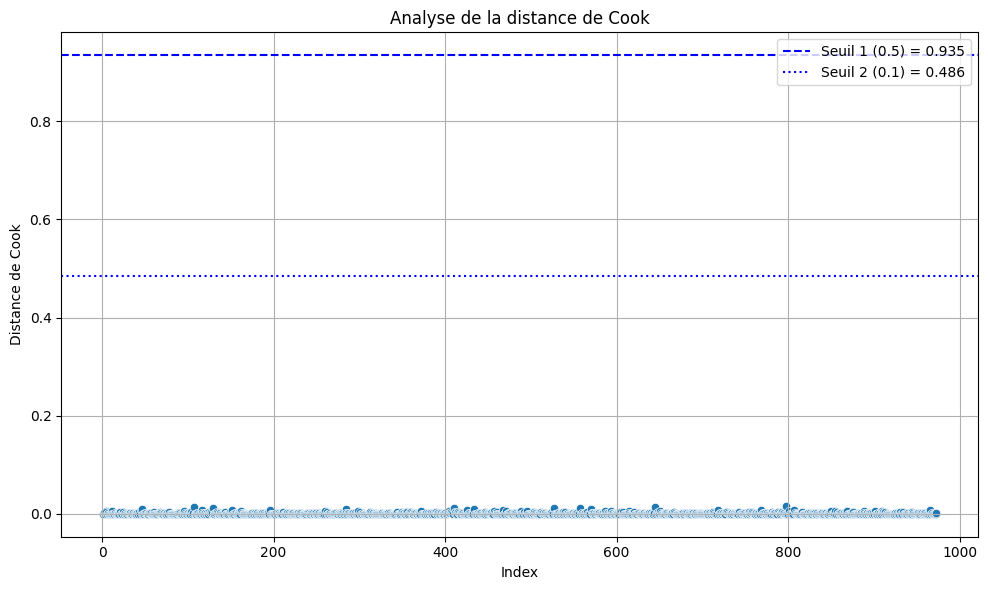
\includegraphics[width=0.7\linewidth]{cook.png}
  \caption{Analyse de la distance de Cook}
\end{figure}

\begin{figure}[H]
  \centering
  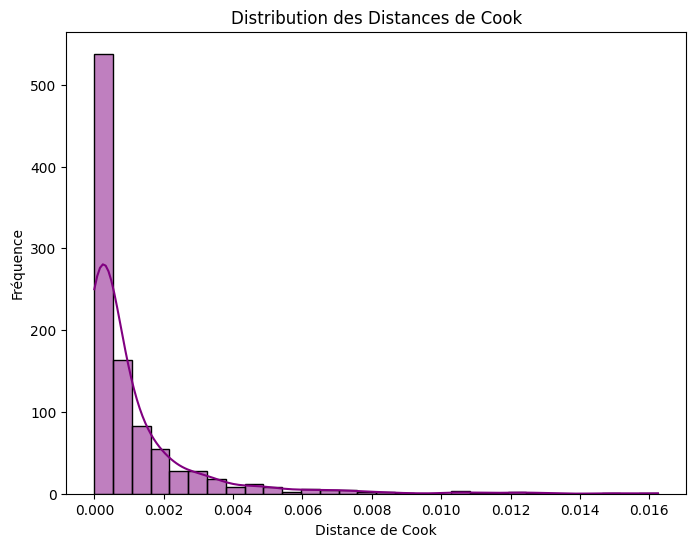
\includegraphics[width=0.7\linewidth]{cooks_d.png}
  \caption{Distribution des distances de Cook}
\end{figure}

\begin{figure}[H]
  \centering
  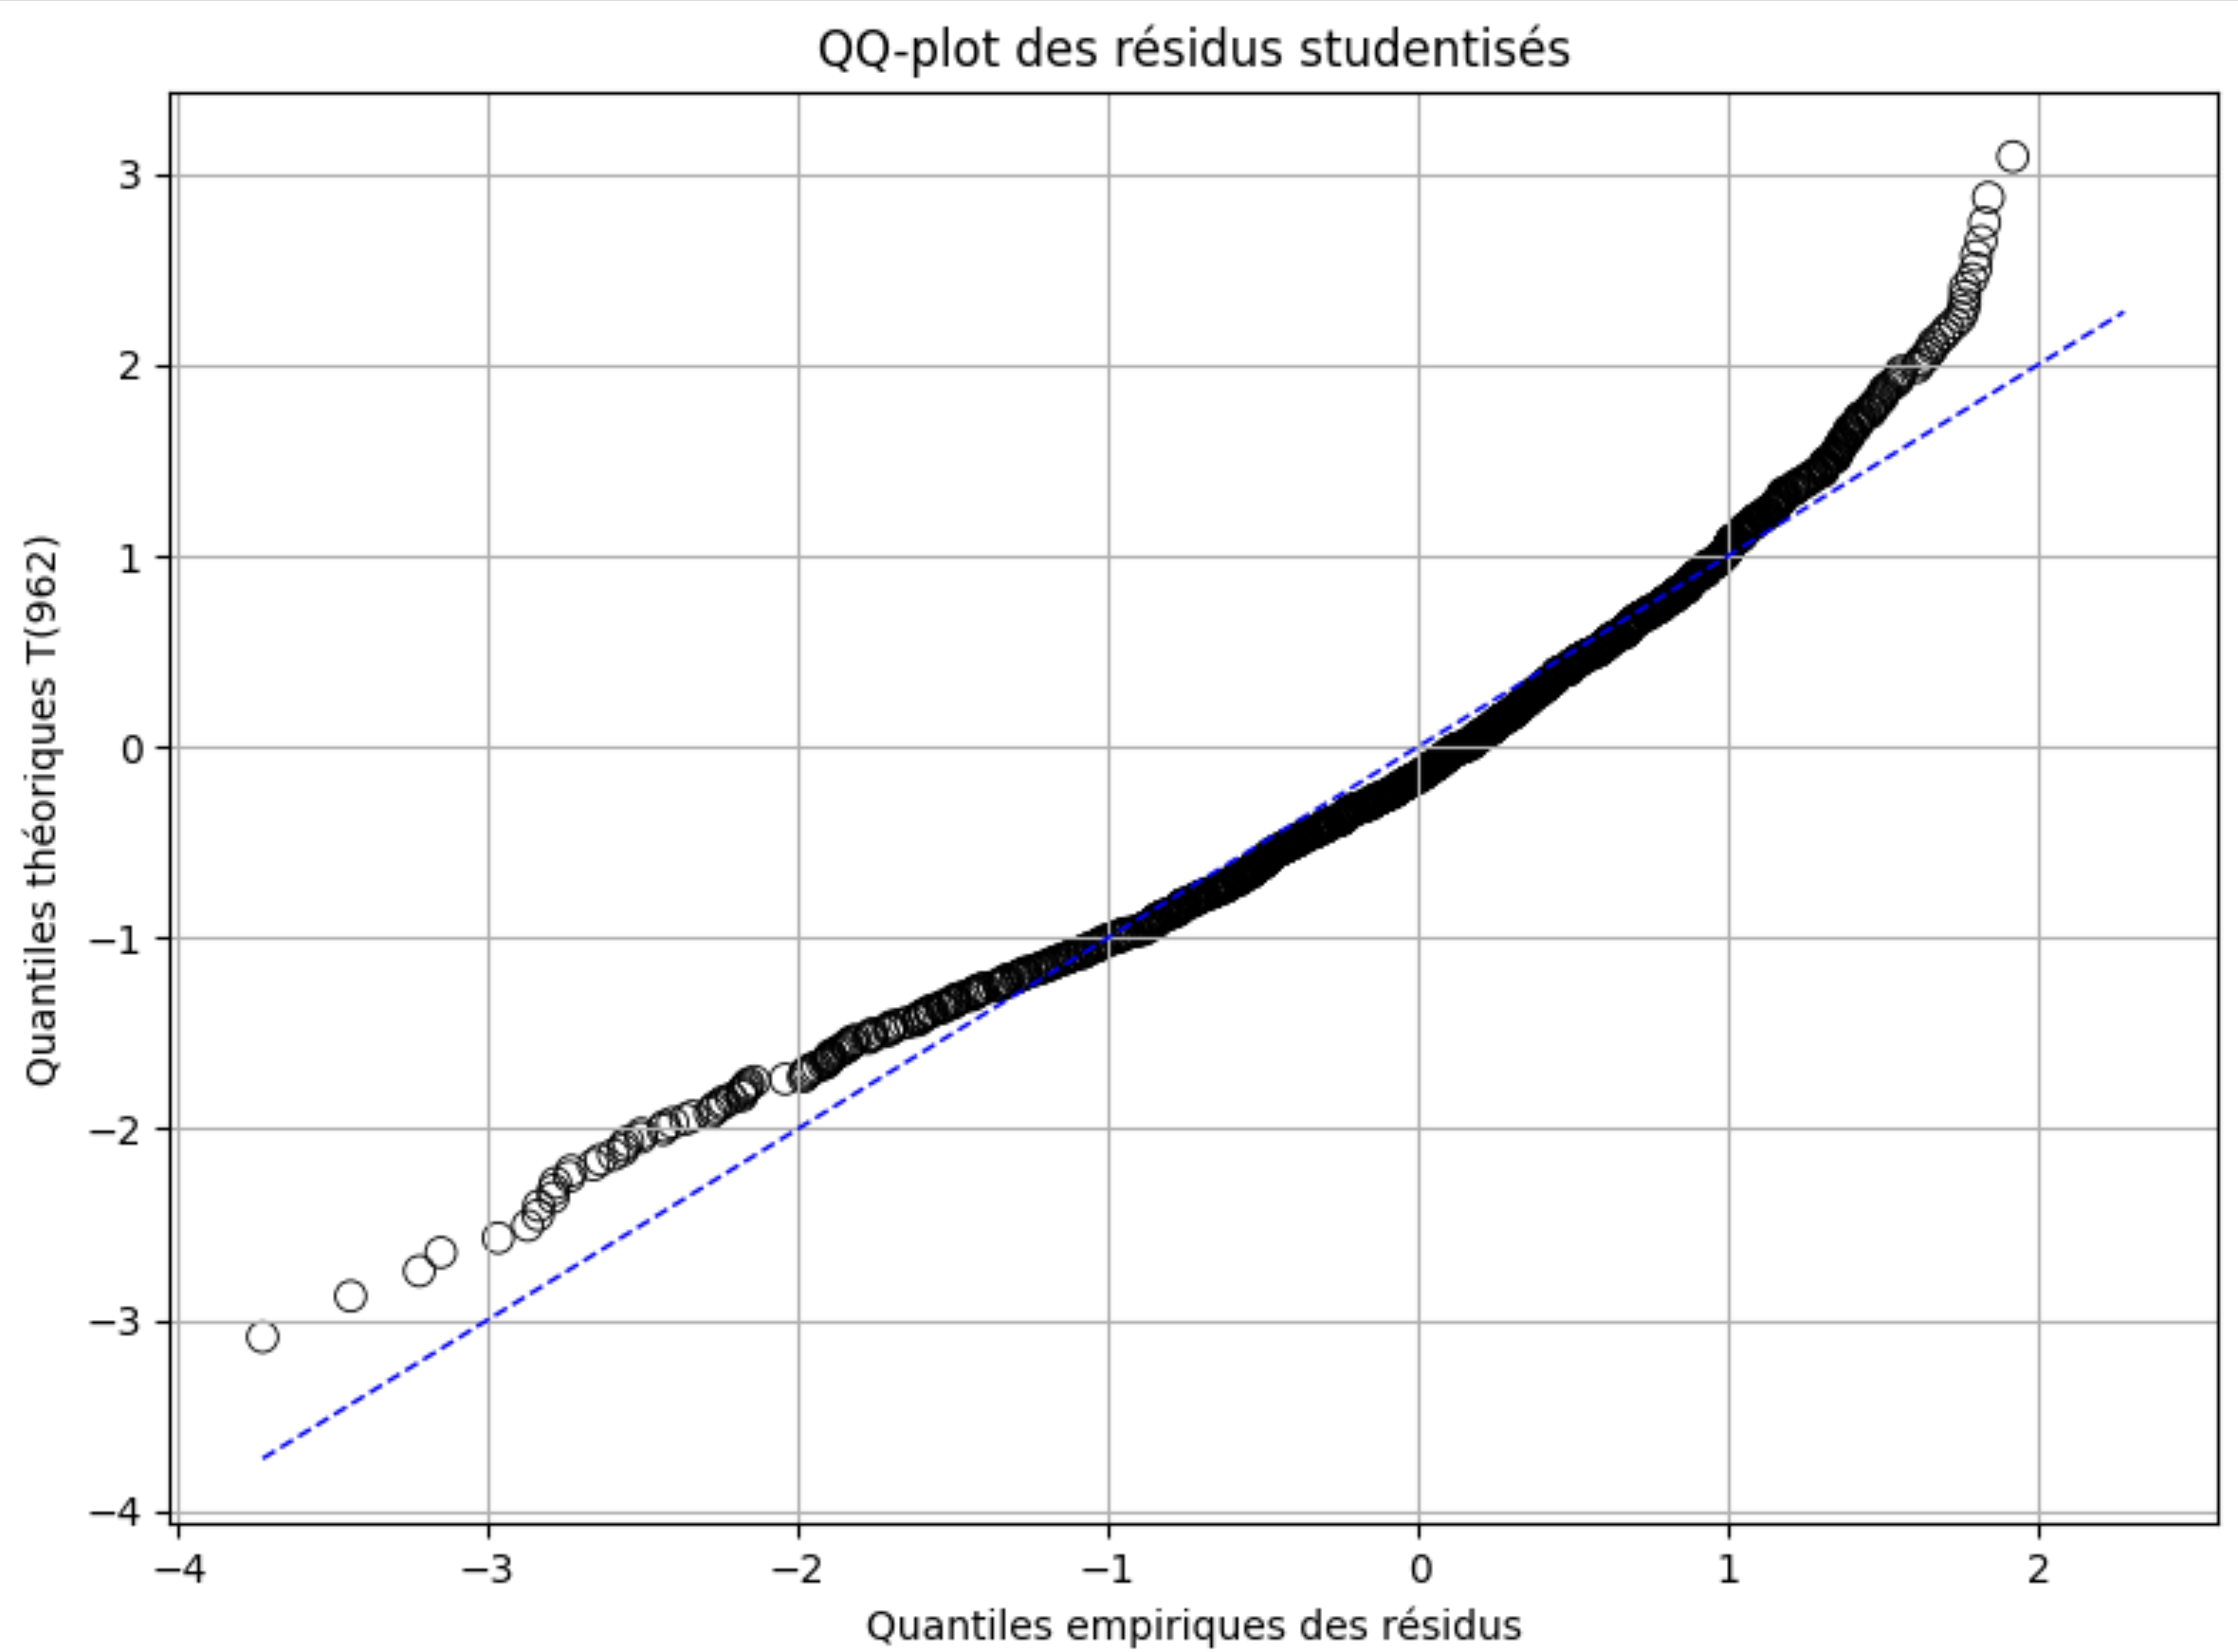
\includegraphics[width=0.7\linewidth]{qqplot.png}
  \caption{QQ-plot des résidus studentisés du modèle final}
\end{figure}

\section{Sélection de modèles supplémentaires}

\subsection{Vérification de la multicolinéarité (VIF)}
Après standardisation, les facteurs d'inflation de la variance (VIF) sont calculés pour chaque prédicteur :

\begin{table}[H]
\centering
\caption{VIF des variables explicatives}
\begin{tabular}{l r}
\toprule
Variable & VIF \\
\midrule
const & 1.00 \\
Age & 1.01 \\
Weight (kg) & 71.43 \\
Height (m) & 20.49 \\
Max\_BPM & 1.01 \\
Avg\_BPM & 1.01 \\
Resting\_BPM & 1.01 \\
Fat\_Percentage & 1.53 \\
Water\_Intake & 1.85 \\
BMI & 63.95 \\
\bottomrule
\end{tabular}
\end{table}

Sur la base de ces résultats, \texttt{Weight} et \texttt{BMI} sont retirés pour stabiliser le modèle.

\subsection{Modèle sans variables colinéaires}
Le modèle réajusté inclut : Age, Avg\_BPM, Resting\_BPM, Fat\_Percentage, Water\_Intake, BMI.
\begin{itemize}
\item $R^2 = 0{,}498$, $R^2_{\text{ajusté}} = 0{,}495$
\item VIF < 2 pour toutes les variables.
\end{itemize}

\subsection{Modèle réduit par élimination pas-à-pas}
Une procédure de ``backward elimination'' retire simultanément Resting\_BPM, Water\_Intake et BMI (p > 0,10). Le modèle final retient :
\begin{itemize}
\item Age, Avg\_BPM, Fat\_Percentage
\end{itemize}
Avec :
\begin{itemize}
\item $R^2 = 0{,}497$, AIC = 2101, BIC = 2120
\item RMSE = 0{,}70, MAE = 0{,}52
\end{itemize}

\section{Recherche exhaustive}
Une recherche exhaustive sur tous les sous-ensembles de variables permet de vérifier la robustesse de la sélection :
\begin{itemize}
\item 511 combinaisons évaluées par AIC, BIC, $R^2$, $R^2_{\text{ajusté}}$.
\item Le meilleur modèle à 4 variables (Age, Height, Avg\_BPM, Fat\_Percentage) présente un AIC minimal ($\sim$2098) et un $R^2_{\text{ajusté}}$ optimal ($\sim$0,499).
\end{itemize}

\begin{figure}[H]
  \centering
  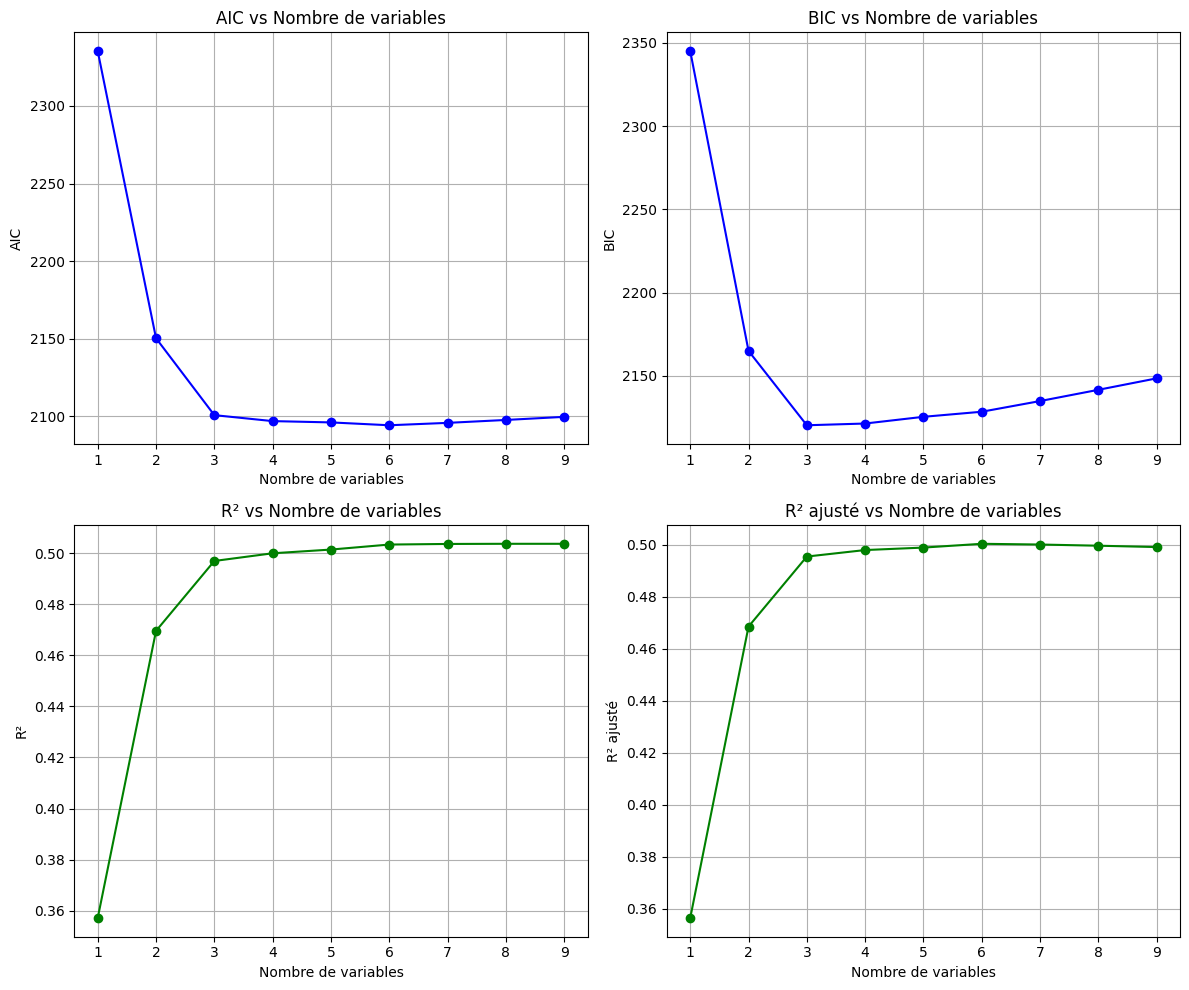
\includegraphics[width=0.7\linewidth]{information_criterion.png}
  \caption{Évolution des Critères de Performance du Modèle en Fonction du Nombre de Variables}
\end{figure}

\section{Validation croisée 10-fold et régularisation}

Validation croisée 10-fold sur les modèles complet, sans colinéarité et réduit :
\begin{itemize}
\item Scores moyens de MSE, MAE, RMSE, $R^2$ très proches entre complet et réduit.
\item Écart-type faible, confirmant la stabilité du modèle réduit.
\end{itemize}

\section{Résultats}

Après ajustement sur les 973 observations, nous évaluons les deux modèles à l’aide des métriques \textit{MSE} et \textit{MAE} :

\begin{itemize}
  \item \textbf{Modèle~1 (toutes les variables)}  
    \begin{itemize}
      \item MSE = 0,4963  
      \item MAE = 0,5569  
    \end{itemize}

  \item \textbf{Modèle~2 (\texttt{Age}, \texttt{Height}, \texttt{Avg\_BPM}, \texttt{Fat\_Percentage})}  
    \begin{itemize}
      \item MSE = 0,5000  
      \item MAE = 0,5595  
    \end{itemize}
\end{itemize}

Visuellement, les nuages de points \emph{prédictions vs. valeurs réelles} pour les deux modèles se superposent presque parfaitement sur la droite d’identité, montrant une dispersion similaire autour de celle-ci.

\bigskip

\noindent\textbf{Interprétation :}  
Le modèle réduit (Modèle~2), composé de seulement quatre prédicteurs, présente une augmentation très légère de l’erreur quadratique moyenne (+0,0037) et de l’erreur absolue moyenne (+0,0026) par rapport au modèle complet. Cette perte minime de précision est largement compensée par la simplicité, la robustesse et la facilité d’interprétation offertes par un nombre réduit de variables. Ainsi, le Modèle~2 constitue un compromis optimal entre performance prédictive et parcimonie.

\begin{figure}[H]
  \centering
  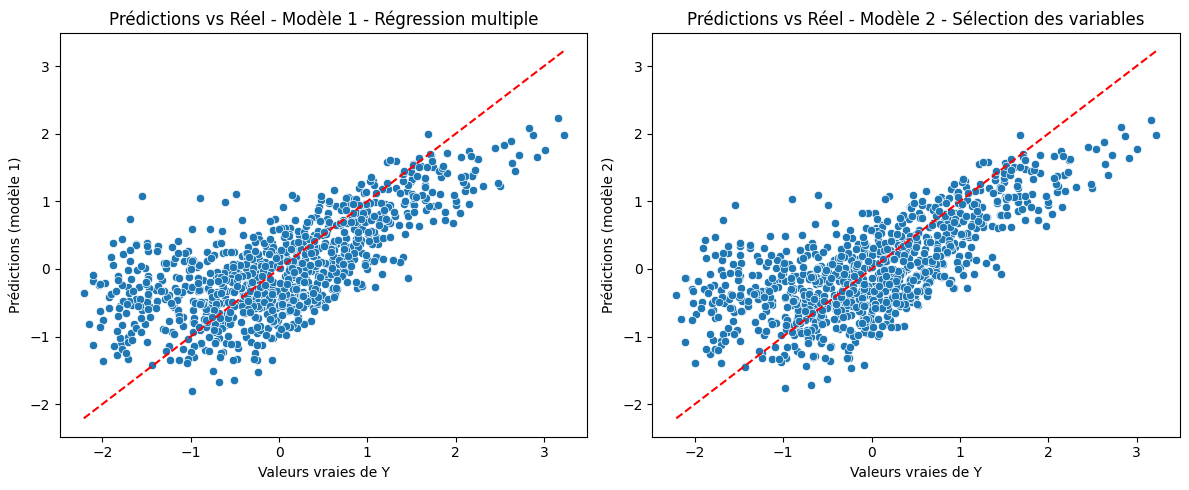
\includegraphics[width=0.7\linewidth]{prediction.png}
  \caption{Comparaison des calories brûlées prédites par les deux modèles}
\end{figure}

\subsection{Équation de prédiction et interprétation des coefficients}

L’équation du modèle final s’écrit :
\begin{multline*}
\widehat{\text{Calories\_Burned}}
=989{,}14-3{,}74\,\text{Age}
-120{,}56\,\text{Height (m)}
+6{,}47\,\text{Avg\_BPM}\\
-26{,}48\,\text{Fat\_Percentage}.
\end{multline*}

\paragraph{Intercept (\(\beta_0 = 989{,}14\))}  
Valeur prédite lorsque toutes les variables explicatives sont nulles. Ici, l’interprétation n’est pas réaliste (âge = 0, taille = 0 m…), mais cet intercept permet d’ajuster correctement le modèle.

\paragraph{Âge (\(\beta_1 = -3{,}74\))}  
Chaque année supplémentaire entraîne en moyenne une diminution de 3,74 kcal, toutes choses égales par ailleurs.

\paragraph{Taille (\(\beta_2 = -120{,}56\))}  
Un mètre de plus est associé à environ 120,56 kcal en moins. Cette valeur contre-intuitive peut résulter d’une corrélation avec d’autres variables (multicolinéarité), à vérifier via la matrice de corrélation ou le VIF.

\paragraph{Fréquence cardiaque moyenne (\(\beta_3 = +6{,}47\))}  
Chaque battement par minute (BPM) supplémentaire augmente la dépense d’environ 6,47 kcal, ce qui reflète l’effet direct de l’intensité de l’exercice.

\paragraph{Pourcentage de masse grasse (\(\beta_4 = -26{,}48\))}  
Un point de pourcentage de masse grasse en plus correspond à une baisse de ~26,48 kcal, probablement en lien avec un métabolisme de base plus faible chez les sujets plus gras.

\section{Conclusion}
En conclusion, ce travail démontre que quatres variables clés suffisent à expliquer près de 50 \% de la variabilité de la dépense calorique en séance de sport, facilitant l’interprétation et le déploiement du modèle. Les coefficients standardisés montrent que la fréquence cardiaque moyenne est le prédicteur le plus influent, suivi négativement par la taille, le pourcentage de masse grasse et l’âge. Ces conclusions offrent une base statistique solide pour adapter les programmes d’entraînement en fonction du profil physiologique des pratiquants. 

\newpage
\end{document}
